\section*{Portable abstraction of hierarchical architectures for high-\/performance computing}





 \hypertarget{index_Introduction}{}\section{Introduction}\label{index_Introduction}
hwloc provides command line tools and a C API to obtain the hierarchical map of key computing elements, such as: NUMA memory nodes, shared caches, processor sockets, processor cores, and processor \char`\"{}threads\char`\"{}. hwloc also gathers various attributes such as cache and memory information, and is portable across a variety of different operating systems and platforms.

hwloc primarily aims at helping high-\/performance computing (HPC) applications, but is also applicable to any project seeking to exploit code and/or data locality on modern computing platforms.

Note that the hwloc project represents the merger of the libtopology project from INRIA and the Portable Linux Processor Affinity (PLPA) sub-\/project from Open MPI. {\itshape Both of these prior projects are now deprecated.\/} The first hwloc release is essentially a \char`\"{}re-\/branding\char`\"{} of the libtopology code base, but with both a few genuinely new features and a few PLPA-\/like features added in. More new features and more PLPA-\/like features will be added to hwloc over time.

hwloc supports the following operating systems:


\begin{DoxyItemize}
\item Linux (including old kernels not having sysfs topology information, with knowledge of cpusets, offline cpus, and Kerrighed support) 
\item Solaris 
\item AIX 
\item Darwin / OS X 
\item OSF/1 (a.k.a., Tru64) 
\item HP-\/UX 
\item Microsoft Windows 
\end{DoxyItemize}

hwloc only reports the number of processors on unsupported operating systems; no topology information is available.

For development and debugging purposes, hwloc also offers the ability to work on \char`\"{}fake\char`\"{} topologies:


\begin{DoxyItemize}
\item Symmetrical tree of resources generated from a list of level arities 
\item Remote machine simulation through the gathering of Linux sysfs topology files 
\end{DoxyItemize}

hwloc can display the topology in a human-\/readable format, either in graphical mode (X11), or by exporting in one of several different formats, including: plain text, PDF, PNG, and FIG (see Examples below). Note that some of the export formats require additional support libraries.

hwloc offers a programming interface for manipulating topologies and objects. It also brings a powerful CPU bitmap API that is used to describe topology objects location on physical/logical processors. See the \hyperlink{index_interface}{Programming interface} below. It may also be used to binding applications onto certain cores or memory nodes. Several utility programs are also provided to ease command-\/line manipulation of topology objects, binding of processes, and so on.

 \hypertarget{index_installation}{}\section{Installation}\label{index_installation}
hwloc (\href{http://www.open-mpi.org/projects/hwloc/}{\tt http://www.open-\/mpi.org/projects/hwloc/}) is available under the BSD license. It is hosted as a sub-\/project of the overall Open MPI project (\href{http://www.open-mpi.org/}{\tt http://www.open-\/mpi.org/}). Note that hwloc does not require any functionality from Open MPI -\/-\/ it is a wholly separate (and much smaller!) project and code base. It just happens to be hosted as part of the overall Open MPI project.

Nightly development snapshots are available on the web site. Additionally, the code can be directly checked out of Subversion:


\begin{DoxyCode}
shell$ svn checkout http://svn.open-mpi.org/svn/hwloc/trunk hwloc-trunk
shell$ cd hwloc-trunk
shell$ ./autogen.sh
\end{DoxyCode}


Note that GNU Autoconf $>$=2.60, Automake $>$=1.10 and Libtool $>$=2.2.6 are required when building from a Subversion checkout.

Installation by itself is the fairly common GNU-\/based process:


\begin{DoxyCode}
shell$ ./configure --prefix=...
shell$ make
shell$ make install
\end{DoxyCode}


The hwloc command-\/line tool \char`\"{}lstopo\char`\"{} produces human-\/readable topology maps, as mentioned above. It can also export maps to the \char`\"{}fig\char`\"{} file format. Support for PDF, Postscript, and PNG exporting is provided if the \char`\"{}Cairo\char`\"{} development package can be found when hwloc is configured and build. Similarly, lstopo's XML support requires the libxml2 development package.

 \hypertarget{index_examples}{}\section{Examples}\label{index_examples}
On a 4-\/socket 2-\/core machine with hyperthreading, the {\ttfamily lstopo} tool may show the following outputs:

 
\begin{DoxyImageNoCaption}
  \mbox{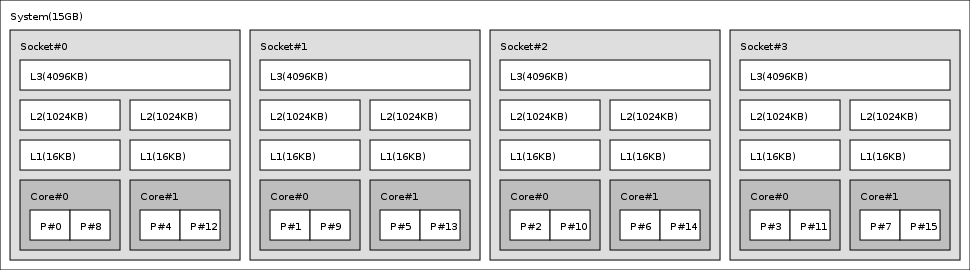
\includegraphics[width=\textwidth]{dudley.png}}
\end{DoxyImageNoCaption}


\begin{DoxyVerb}
System(15GB)
  Socket#0 + L3(4096KB)
    L2(1024KB) + L1(16KB) + Core#0
      P#0
      P#8
    L2(1024KB) + L1(16KB) + Core#1
      P#4
      P#12
  Socket#1 + L3(4096KB)
    L2(1024KB) + L1(16KB) + Core#0
      P#1
      P#9
    L2(1024KB) + L1(16KB) + Core#1
      P#5
      P#13
  Socket#2 + L3(4096KB)
    L2(1024KB) + L1(16KB) + Core#0
      P#2
      P#10
    L2(1024KB) + L1(16KB) + Core#1
      P#6
      P#14
  Socket#3 + L3(4096KB)
    L2(1024KB) + L1(16KB) + Core#0
      P#3
      P#11
    L2(1024KB) + L1(16KB) + Core#1
      P#7
      P#15
\end{DoxyVerb}


On a 4-\/socket 2-\/core Opteron NUMA machine, the {\ttfamily lstopo} tool may show the following outputs:

 
\begin{DoxyImageNoCaption}
  \mbox{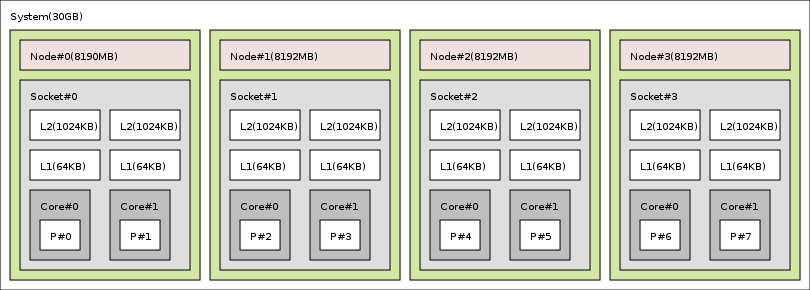
\includegraphics[width=\textwidth]{hagrid.png}}
\end{DoxyImageNoCaption}


\begin{DoxyVerb}
System(62GB)
  Node#0(8190MB) + Socket#0
    L2(1024KB) + L1(64KB) + Core#0 + P#0
    L2(1024KB) + L1(64KB) + Core#1 + P#1
  Node#1(8192MB) + Socket#1
    L2(1024KB) + L1(64KB) + Core#0 + P#2
    L2(1024KB) + L1(64KB) + Core#1 + P#3
  Node#2(8192MB) + Socket#2
    L2(1024KB) + L1(64KB) + Core#0 + P#4
    L2(1024KB) + L1(64KB) + Core#1 + P#5
  Node#3(8192MB) + Socket#3
    L2(1024KB) + L1(64KB) + Core#0 + P#6
    L2(1024KB) + L1(64KB) + Core#1 + P#7
  Node#4(8192MB) + Socket#4
    L2(1024KB) + L1(64KB) + Core#0 + P#8
    L2(1024KB) + L1(64KB) + Core#1 + P#9
  Node#5(8192MB) + Socket#5
    L2(1024KB) + L1(64KB) + Core#0 + P#10
    L2(1024KB) + L1(64KB) + Core#1 + P#11
  Node#6(8192MB) + Socket#6
    L2(1024KB) + L1(64KB) + Core#0 + P#12
    L2(1024KB) + L1(64KB) + Core#1 + P#13
  Node#7(8192MB) + Socket#7
    L2(1024KB) + L1(64KB) + Core#0 + P#14
    L2(1024KB) + L1(64KB) + Core#1 + P#15
\end{DoxyVerb}


On a 2-\/socket quad-\/core Xeon (pre-\/Nehalem, with 2 dual-\/core dies into each socket):

 
\begin{DoxyImageNoCaption}
  \mbox{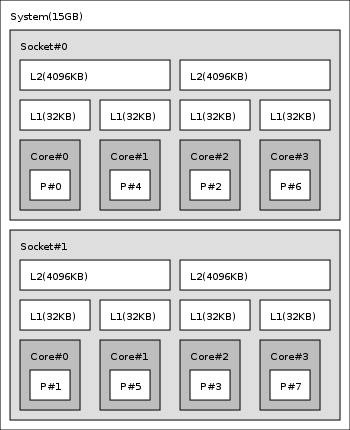
\includegraphics[width=8cm]{emmett.png}}
\end{DoxyImageNoCaption}


\begin{DoxyVerb}
System(15GB)
  Socket#0
    L2(4096KB)
      L1(32KB) + Core#0 + P#0
      L1(32KB) + Core#1 + P#4
    L2(4096KB)
      L1(32KB) + Core#2 + P#2
      L1(32KB) + Core#3 + P#6
  Socket#1
    L2(4096KB)
      L1(32KB) + Core#0 + P#1
      L1(32KB) + Core#1 + P#5
    L2(4096KB)
      L1(32KB) + Core#2 + P#3
      L1(32KB) + Core#3 + P#7
\end{DoxyVerb}


\hypertarget{index_interface}{}\section{Programming interface}\label{index_interface}
The basic interface is available in \hyperlink{hwloc_8h_source}{hwloc.h}. It mostly offers low-\/level routines for advanced programmers that want to manually manipulate objects and follow links between them. Developers should look at \hyperlink{helper_8h_source}{hwloc/helper.h}, which provides good higher-\/level topology traversal examples.

Each object contains a cpuset describing the list of processors that it contains. These cpusets may be used for \hyperlink{group__hwlocality__binding}{Binding}. hwloc offers an extensive cpuset manipulation interface in \hyperlink{cpuset_8h_source}{hwloc/cpuset.h}.

Moreover, hwloc also comes with additional helpers for interoperability with several commonly used environments. For Linux, some specific helpers are available in \hyperlink{linux_8h_source}{hwloc/linux.h}, and \hyperlink{linux-libnuma_8h_source}{hwloc/linux-\/libnuma.h} if using libnuma. On glibc-\/based systems, additional helpers are available in \hyperlink{glibc-sched_8h_source}{hwloc/glibc-\/sched.h}. For Linux systems with the OpenFabrics verbs library, some dedicated helpers are provided in \hyperlink{openfabrics-verbs_8h_source}{hwloc/openfabrics-\/verbs.h} (this helper file is not yet useful on non-\/Linux systems with the OpenFabrics verbs library).

To precisely define the vocabulary used by hwloc, a \hyperlink{index_glossary}{Glossary} is available and should probably be read first.

Further documentation is available in a full set of HTML pages, man pages, and self-\/contained PDF files (formatted for both both US letter and A4 formats) in the source tarball in doc/doxygen-\/doc/. If you are building from a Subversion checkout, you will need to have Doxygen and pdflatex installed -\/-\/ the documentation will be built during the normal \char`\"{}make\char`\"{} process. The documentation is installed during \char`\"{}make
install\char`\"{} to \$prefix/share/doc/hwloc/ and your systems default man page tree (under \$prefix, of course).

The following section presents an example of API usage.\hypertarget{index_interface_example}{}\section{API example}\label{index_interface_example}
The following small C example (named ``hwloc-\/hello.c'') prints the topology of the machine and bring the process to the first processor of the second core of the machine.


\begin{DoxyCodeInclude}
/* Example hwloc API program.
 *
 * Copyright © 2009 INRIA, Université Bordeaux 1
 * Copyright © 2009 Cisco Systems, Inc.  All rights reserved.
 *
 * hwloc-hello.c 
 */

#include <hwloc.h>

static void print_children(hwloc_topology_t topology, hwloc_obj_t obj, 
                           int depth)
{
    char string[128];
    int i;

    hwloc_obj_snprintf(string, sizeof(string), topology, obj, "#", 0);
    printf("%*s%s\n", 2*depth, "", string);
    for (i = 0; i < obj->arity; i++) {
        print_children(topology, obj->children[i], depth + 1);
    }
}

int main(int argc, char **argv)
{
    int depth, i;
    char string[128];
    unsigned int topodepth;
    hwloc_topology_t topology;
    hwloc_cpuset_t cpuset;
    hwloc_obj_t obj;

    /* Allocate and initialize topology object. */
    hwloc_topology_init(&topology);

    /* ... Optionally, put detection configuration here to e.g. ignore
       some objects types, define a synthetic topology, etc....  

       The default is to detect all the objects of the machine that
       the caller is allowed to access.  See Configure Topology
       Detection. */

    /* Perform the topology detection. */
    hwloc_topology_load(topology);

    /* Optionally, get some additional topology information
       in case we need the topology depth later. */
    topodepth = hwloc_topology_get_depth(topology);

    /* Walk the topology with an array style, from level 0 (always the
       system level) to the lowest level (always the proc level). */
    for (depth = 0; depth < topodepth; depth++) {
        printf("*** Objects at level %d\n", depth);
        for (i = 0; i < hwloc_get_nbobjs_by_depth(topology, depth); 
             i++) {
            hwloc_obj_snprintf(string, sizeof(string), topology,
                       hwloc_get_obj_by_depth(topology, depth, i),
                       "#", 0);
            printf("Index %d: %s\n", i, string);
        }
    }

    /* Walk the topology with a tree style. */
    printf("*** Printing overall tree\n");
    print_children(topology, hwloc_get_system_obj(topology), 0);

    /* Print the number of sockets. */
    depth = hwloc_get_type_depth(topology, HWLOC_OBJ_SOCKET);
    if (depth == HWLOC_TYPE_DEPTH_UNKNOWN) {
        printf("*** The number of sockets is unknown\n");
    } else {
        printf("*** %u socket(s)\n", 
               hwloc_get_nbobjs_by_depth(topology, depth));
    }

    /* Find out where cores are, or else smaller sets of CPUs if 
       the OS doesn't have the notion of a "core". */
    depth = hwloc_get_type_or_below_depth(topology, HWLOC_OBJ_CORE);

    /* Get last level. */
    obj = hwloc_get_obj_by_depth(topology, depth, 
                   hwloc_get_nbobjs_by_depth(topology, depth) - 1);
    if (obj) {
        /* Get a copy of its cpuset that we may modify. */
        cpuset = hwloc_cpuset_dup(obj->cpuset);
    
        /* Get only one logical processor (in case the core is
           SMT/hyperthreaded). */
        hwloc_cpuset_singlify(cpuset);

        /* And try to bind ourself there. */
        if (hwloc_set_cpubind(topology, cpuset, 0)) {
            char *str;
            hwloc_cpuset_asprintf(&str, obj->cpuset);
            printf("Couldn't bind to cpuset %s\n", str);
            free(str);
        }

        /* Free our cpuset copy */
        hwloc_cpuset_free(cpuset);
    }

    /* Destroy topology object. */
    hwloc_topology_destroy(topology);

    return 0;
}
\end{DoxyCodeInclude}


hwloc provides a {\ttfamily pkg-\/config} executable to obtain relevant compiler and linker flags. For example, it can be used thusly to compile applications that utilize the hwloc library (assuming GNU Make):

\begin{DoxyVerb}
CFLAGS += $(pkg-config --cflags hwloc)
LDLIBS += $(pkg-config --libs hwloc)
cc hwloc-hello.c $(CFLAGS) -o hwloc-hello $(LDLIBS)
\end{DoxyVerb}


On a machine with 4GB of RAM and 2 processor sockets -\/-\/ each socket of which has two processor cores -\/-\/ the output from running {\ttfamily hwloc-\/hello} could be something like the following:

\begin{DoxyVerb}
shell$ ./hwloc-hello
*** Objects at level 0
Index 0: System(3938MB)
*** Objects at level 1
Index 0: Socket#0
Index 1: Socket#1
*** Objects at level 2
Index 0: Core#0
Index 1: Core#1
Index 2: Core#3
Index 3: Core#2
*** Objects at level 3
Index 0: P#0
Index 1: P#1
Index 2: P#2
Index 3: P#3
*** Printing overall tree
System(3938MB)
  Socket#0
    Core#0
      P#0
    Core#1
      P#1
  Socket#1
    Core#3
      P#2
    Core#2
      P#3
*** 2 socket(s)
shell$ 
\end{DoxyVerb}


 \hypertarget{index_bugs}{}\section{Questions and bugs}\label{index_bugs}
Questions should be sent to the devel mailing list (\href{http://www.open-mpi.org/community/lists/hwloc.php}{\tt http://www.open-\/mpi.org/community/lists/hwloc.php}). Bug reports should be reported in the tracker (\href{https://svn.open-mpi.org/trac/hwloc/}{\tt https://svn.open-\/mpi.org/trac/hwloc/}).

 \hypertarget{index_history}{}\section{History / credits}\label{index_history}
hwloc is the evolution and merger of the libtopology (\href{http://runtime.bordeaux.inria.fr/libtopology/}{\tt http://runtime.bordeaux.inria.fr/libtopology/}) project and the Portable Linux Processor Affinity (PLPA) (\href{http://www.open-mpi.org/projects/plpa/}{\tt http://www.open-\/mpi.org/projects/plpa/}) project. Because of functional and ideological overlap, these two code bases and ideas were merged and released under the name \char`\"{}hwloc\char`\"{} as an Open MPI sub-\/project.

libtopology was initially developed by the INRIA Runtime Team-\/Project (\href{http://runtime.bordeaux.inria.fr/}{\tt http://runtime.bordeaux.inria.fr/}) (headed by Raymond Namyst (\href{http://dept-info.labri.fr/~namyst/}{\tt http://dept-\/info.labri.fr/$\sim$namyst/}). PLPA was initially developed by the Open MPI development team as a sub-\/project. Both are now deprecated in favor of hwloc, which is distributed as an Open MPI sub-\/project.

\hypertarget{index_glossary}{}\section{Glossary}\label{index_glossary}

\begin{DoxyDescription}
\item[Object ]Interesting kind of part of the system, such as a Core, a Cache, a Memory node, etc. The different types detected by hwloc are detailed in the \hyperlink{group__hwlocality__types_gacd37bb612667dc437d66bfb175a8dc55}{hwloc\_\-obj\_\-type\_\-t} enumeration.

They are topologically sorted by CPU set into a tree whose root is the System object (which always exists). 


\item[CPU set ]The set of logical processors logically included in an object (if any). This term does {\itshape not\/} have any relation to an operating system ``CPU set.''


\item[Father object ]The object logically containing the current object, for example because its CPU set includes the CPU set of the current object.


\item[Children object(s) ]The object (or objects) contained in the current object because their CPU set is included in the CPU set of the current object.


\item[Arity ]The number of children of an object.


\item[Sibling objects ]Objects of the same type which have the same father.


\item[Sibling rank ]Index to uniquely identify objects of the same type which have the same father, and is always in the range \mbox{[}0, fathers\_\-arity).


\item[Cousin objects ]Objects of the same type as the current object.


\item[Level ]Set of objects of the same type.


\item[OS index ]The index that the operating system (OS) uses to identify the object. This may be completely arbitrary, or it may depend on the BIOS configuration.


\item[Depth ]Nesting level in the object tree, starting from the 0th object (i.e., the System object).


\item[Logical index ]Index to uniquely identify objects of the same type. It is generally used to express proximity. This index is always linear and in the range \mbox{[}0, num\_\-objs\_\-same\_\-type\_\-same\_\-level). Think of it as ``cousin rank.''


\end{DoxyDescription}

The following diagram can help to understand the vocabulary of the relationships by showing the example of a machine with two dual core sockets (with no hardware threads); thus, a topology with 4 levels.

 
\begin{DoxyImageNoCaption}
  \mbox{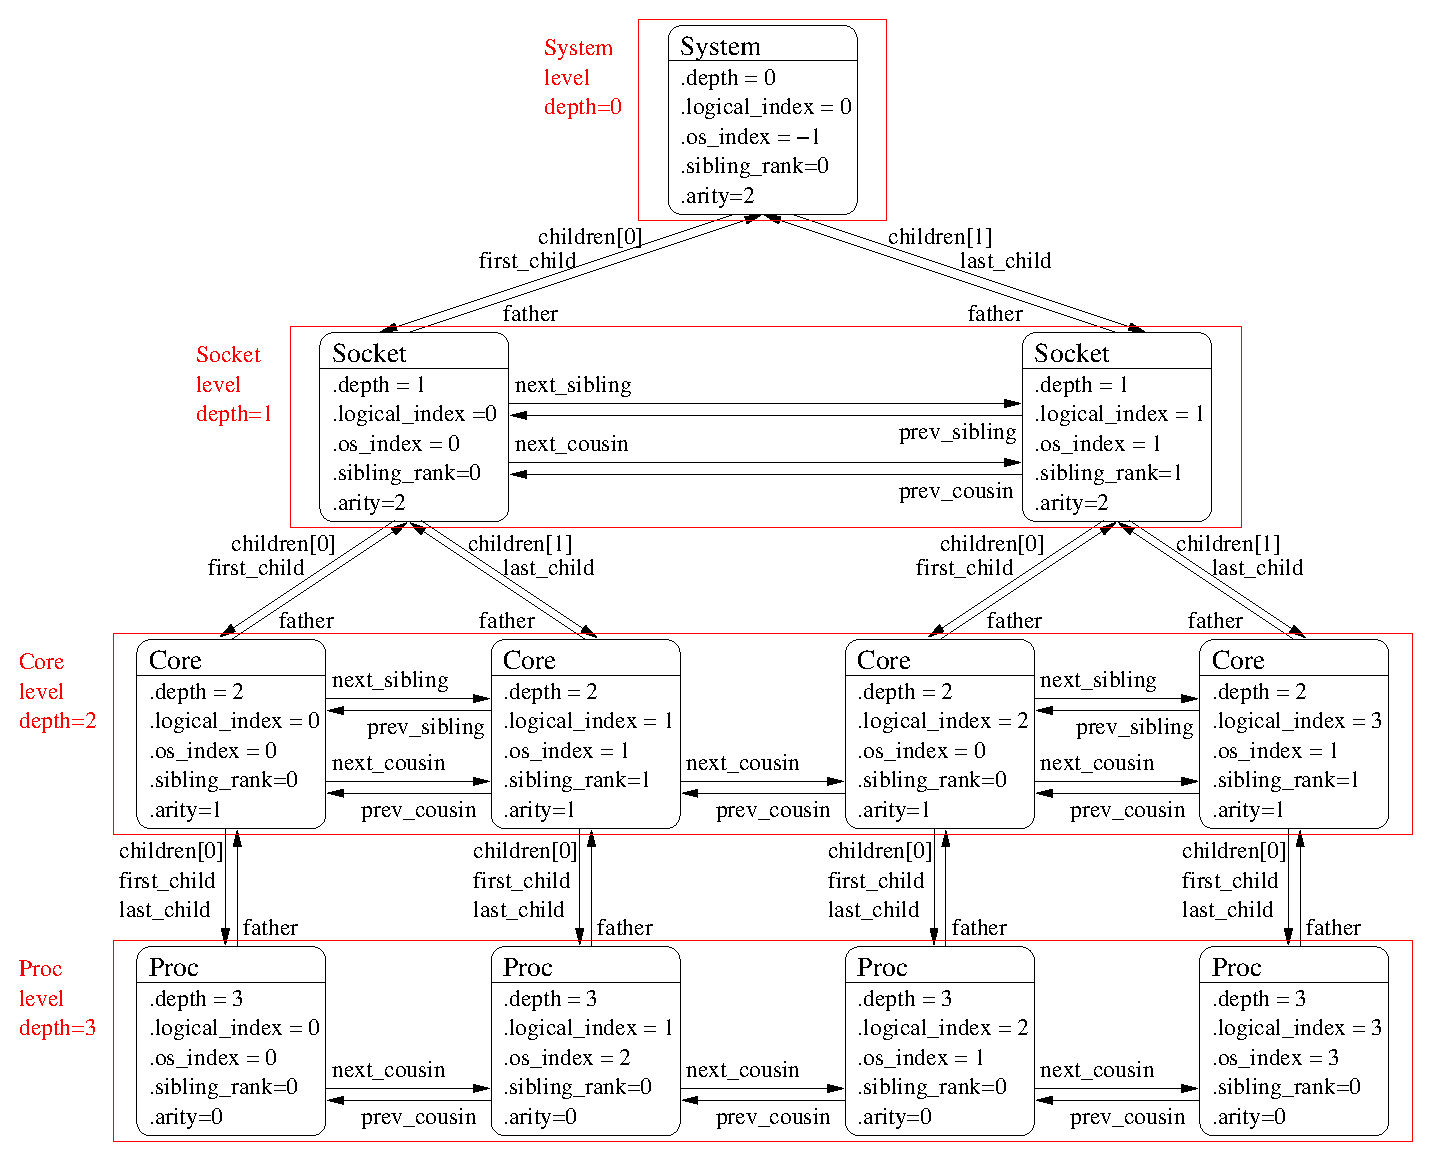
\includegraphics[width=\textwidth]{diagram}}
\end{DoxyImageNoCaption}


It should be noted that for Processor objects, the logical index -\/-\/ as computed linearly by hwloc -\/-\/ is not the same as the OS index. 
